
The random library provides a selection of random number generators, each with different strategies and properties. In this recipe, we examine a function to compare the different options by creating a histogram of their output.

\subsubsection{How to do it…}

In this recipe, we compare the different random number generators provided by the C++ random library:

\begin{itemize}
\item 
We start with some constants to provide uniform parameters for the random number generators:

\begin{lstlisting}[style=styleCXX]
constexpr size_t n_samples{ 1000 };
constexpr size_t n_partitions{ 10 };
constexpr size_t n_max{ 50 };
\end{lstlisting}

n\_samples is the number of samples to examine, n\_partitions is the number of partitions in which to display the samples, and n\_max is the maximum size of a bar in the histogram (this will vary some due to rounding).

These numbers provide a reasonable display of the differences between the engines. Increasing the ratio of samples versus partitions tends to smooth out the curves and obscure the differences between the engines.

\item 
This is the function that collects random number samples and displays a histogram:

\begin{lstlisting}[style=styleCXX]
template <typename RNG>
void histogram(const string_view& rng_name) {
	auto p_ratio = (double)RNG::max() / n_partitions;
	RNG rng{}; // construct the engine object
	
	// collect the samples
	vector<size_t> v(n_partitions);
	for(size_t i{}; i < n_samples; ++i) {
		++v[rng() / p_ratio];
	}

	// display the histogram
	auto max_el = std::max_element(v.begin(),
		v.end());
	auto v_ratio = *max_el / n_max;
	if(v_ratio < 1) v_ratio = 1;
	cout << format("engine: {}\n", rng_name);
	for(size_t i{}; i < n_partitions; ++i) {
		cout << format("{:02}:{:*<{}}\n",
			i + 1, ' ', v[i] / v_ratio);
	}
	cout << '\n';
}
\end{lstlisting}


In a nutshell, this function stores a histogram of collected samples in a vector. It then displays the histogram as a series of asterisks on the console.

\item 
We call histogram() from main(), like this:

\begin{lstlisting}[style=styleCXX]
int main() {
	histogram<std::random_device>("random_device");
	histogram<std::default_random_engine>
		("default_random_engine");
	histogram<std::minstd_rand0>("minstd_rand0");
	histogram<std::minstd_rand>("minstd_rand");
	histogram<std::mt19937>("mt19937");
	histogram<std::mt19937_64>("mt19937_64");
	histogram<std::ranlux24_base>("ranlux24_base");
	histogram<std::ranlux48_base>("ranlux48_base");
	histogram<std::ranlux24>("ranlux24");
	histogram<std::ranlux48>("ranlux48");
	histogram<std::knuth_b>("knuth_b");
}
\end{lstlisting}

Output:

\begin{center}
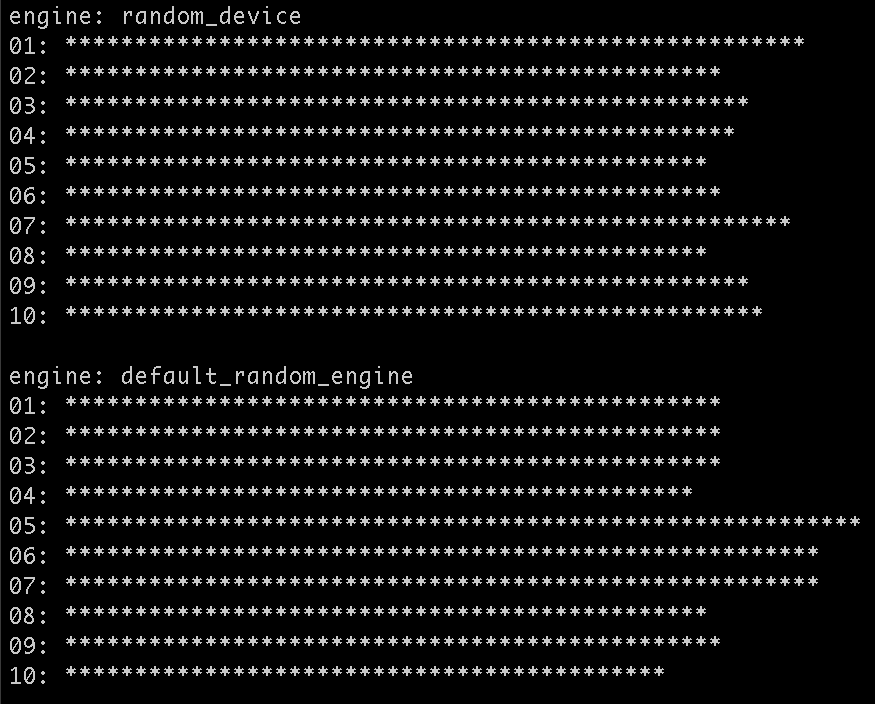
\includegraphics[width=0.8\textwidth]{content/chapter8/images/1.png}\\
Figure 8.1 – A screenshot of output from the first two random number engines
\end{center}

This screenshot shows histograms of the first two random number engines. Your output will vary.

If we raise the value of n\_samples to 100,000, you'll see that the variance between engines becomes more difficult to discern:

\begin{center}
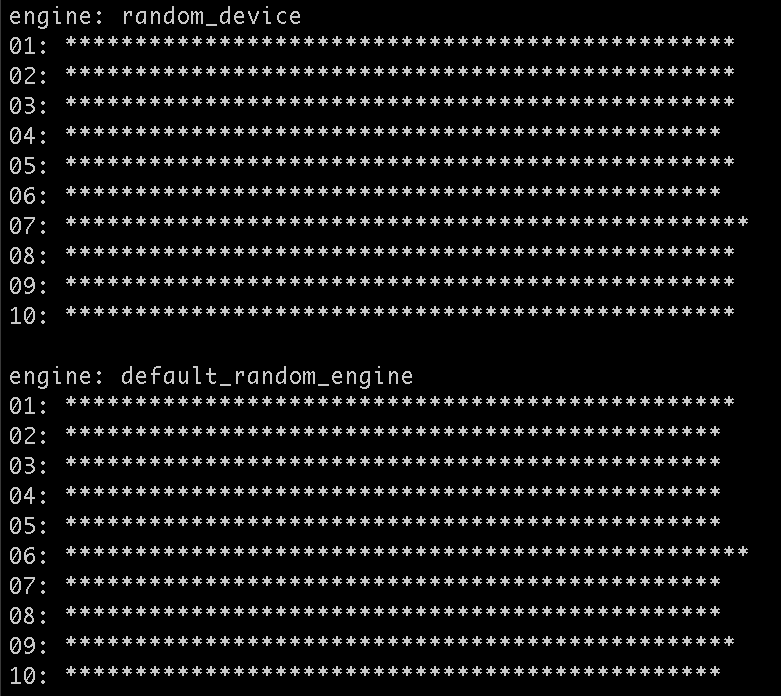
\includegraphics[width=0.8\textwidth]{content/chapter8/images/2.png}\\
Figure 8.2 – A screenshot of output with 100,000 samples
\end{center}

\end{itemize}

\subsubsection{How it works…}

Each of the random number engines has a functor interface that returns the next random number in the sequence:

\begin{lstlisting}[style=styleCXX]
result_type operator()();
\end{lstlisting}

The functor returns a random value, evenly distributed between the min() and max() values. All the random number engines have this interface in common.

The histogram() function takes advantage of this uniformity by using the class of the random number engine in a template:

\begin{lstlisting}[style=styleCXX]
template <typename RNG>
\end{lstlisting}

(RNG is a common abbreviation for Random Number Generator. The library documentation refers to these classes as engines, which is synonymous with RNG for our purposes.) 

We instantiate an object with the RNG class and create a histogram in a vector:

\begin{lstlisting}[style=styleCXX]
RNG rng{};
vector<size_t> v(n_partitions);
for(size_t i{}; i < n_samples; ++i) {
	++v[rng() / p_ratio];
}
\end{lstlisting}

This allows us to easily compare the results of the various random number engines with this technique.


\subsubsection{There's more…}

Each of the random number engines in the library have different methodologies and characteristics. When you run the histogram multiple times, you'll notice that most of the engines have the same distribution each time they're run. That's because they are deterministic – that is, they generate the same sequence of numbers each time. std::random\_device is non-deterministic on most systems. You can use it to seed one of the other engines if you need more variation. It is also common to seed an RNG with the current date and time.

The std::default\_random\_engine is a suitable choice for most purposes.


















